%! TEX root = ../main.tex
% ==============================================================
% IMMUTABLE — generated automatically, do not edit this block
%
% — Provenance ───────────────────────────────────────────────────
%   script            : analysis_scratch/wind_decay_timeseries.py
%   computed_in       : analysis_scratch/wind_decay_timeseries.py
%   plot_type         : wind_transition_timeseries
%   data_class        : DELEG
%   generated_at      : 2026-05-01T12:22:07
%   findings_doc      : (none)
%
% — Thesis context ──────────────────────────────────────────────
%   chapter           : 04
%   caption_label     : fig:ch04_wind_transition_overview
%   caption_short     : 
%
% — Filters ────────────────────────────────────────────────────
%   panel             : 
%   wind              : transition
%   amplitude [V]     : 
%   frequency [Hz]    : 
%   probes            : 
%   run_category      : 
%   quality_flag      : 
%   mooring           : 
%
% — Data provenance ────────────────────────────────────────────
%   n_runs            : 
%   in_probes_used    : 
%   out_probes_used   : 
%   probe_configs     : 
%   non_final_config_n: 
%   datasets        :
%     PROCESSED-20251005-sixttry6roof-highMooring
%     PROCESSED-20251110-tett6roof-lowM-ekte580
%     PROCESSED-20251110-tett6roof-lowMooring
%     PROCESSED-20251110-tett6roof-lowMooring-2
%     PROCESSED-20251112-tett6roof
%     PROCESSED-20251113-tett6roof
%     PROCESSED-20251113-tett6roof-loosepaneltaped
%     PROCESSED-20251113-tett6roof-probeadjusted
%     PROCESSED-20260305-newProbePos-tett6roof
%     PROCESSED-20260306-newProbePos-tett6roof
%     PROCESSED-20260307-ProbPos4_31_FPV_2-tett6roof
%     PROCESSED-20260312-ProbPos4_31_FPV_2-tett6roof
%     PROCESSED-20260313-ProbePos4_31_FPV_2-tett6roof
%     PROCESSED-20260314-ProbePos4_31_FPV_2-tett6roof
%     PROCESSED-20260316-ProbePos4_31_FPV_2-tett6roof
%     PROCESSED-20260316-ProbePos4_31_FPV_2-tett6roof-under9Mooring
%     PROCESSED-20260319-ProbePos4_31_FPV_2-tett6roof-under9Mooring
%     PROCESSED-20260321-ProbePos4_31_FPV_2-tett6roof-under9Mooring-height100-RENAMED
%     PROCESSED-20260323-ProbePos4_31_FPV_2-tett6roof-under9Mooring-height100
%     PROCESSED-20260323-ProbePos4_31_FPV_2-tett6roof-under9Mooring-height136
%     PROCESSED-20260324-ProbePos4_31_FPV_2-tett6roof-under9Mooring-height100
%     PROCESSED-20260325-ProbePos4_31_FPV_2-tett6roof-under9Mooring-height100
%     PROCESSED-20260326-ProbePos4_31_FPV_2-tett6roof-under9Mooring-height100
%     PROCESSED-20260326-ProbePos4_31_FPV_2-tett6roof-under9Mooring-height100-lowrange
%     PROCESSED-20260327-ProbePos4_31_FPV_2-tett6roof-under9Mooring30-height100-lowrange
%   run_paths       :
%     (omitted — aggregate over > threshold runs, see datasets)
%
% — Method / numerical parameters ─────────────────────────────
%   grouper           : 
%   collapse_panels   : 
%   fft_window_hz     : 
%   extra_params      : Two single-run time-series. Wind ramp-up = 20260314 fullpanel-fromZeroWinToMaxWin-run1.csv (probe config march2026_better_rearranging). Wind decay   = 20260327 experimental-fromMaxToZeroWin-depth580-mstop30-run-endofday.csv (same probe config). Probes shown: IN=9373/170 (colour #FEA11B amber, fully exposed to wind), OUT=12400/250 (colour #2EC483 green, sheltered behind panel). Per-probe baseline μ₀ subtracted: ramp-up = mean of first 2 s (tank at rest before fan); decay = mean of last 2 s (tank settled by ~23 min). Y-axis clipped to ±15 mm so the wind-setup tilt and chop envelope are readable on the same scale across all four panels. Subfigure order top→bottom: ramp-up full record (minutes), ramp-up first 60 s (seconds), decay full record (minutes), decay first 60 s (seconds).
%
% — Summary stats cited in caption ────────────────────────────
%   (none registered — pass extra_stats=... to build_fig_meta)
%
% — Subfigures available ───────────────────────────────────────
%     FIGURES/ch04_wind_rampup_full.pdf
%     FIGURES/ch04_wind_rampup_zoom60.pdf
%     FIGURES/ch04_wind_decay_full.pdf
%     FIGURES/ch04_wind_decay_zoom60.pdf
% ── end immutable block ─────────────────────────────────────────
\begin{figure}[p]
  \centering
  \begin{subfigure}[b]{1.0\linewidth}
    \centering
    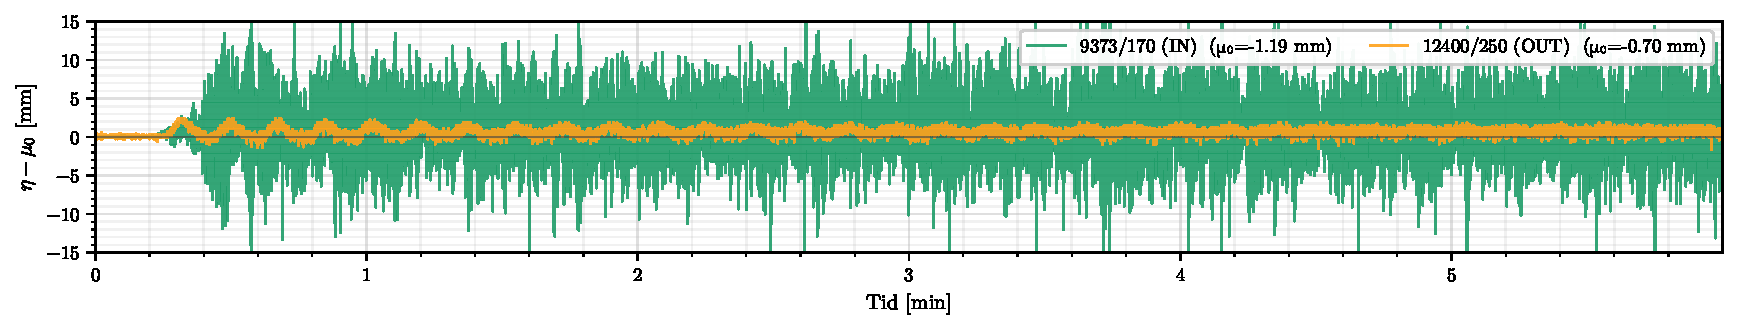
\includegraphics[width=\linewidth]{FIGURES/ch04_wind_rampup_full.pdf}
    \caption{TODO}
    \label{fig:ch04_wind_rampup_full}
  \end{subfigure}
  \\[1ex]
  \begin{subfigure}[b]{1.0\linewidth}
    \centering
    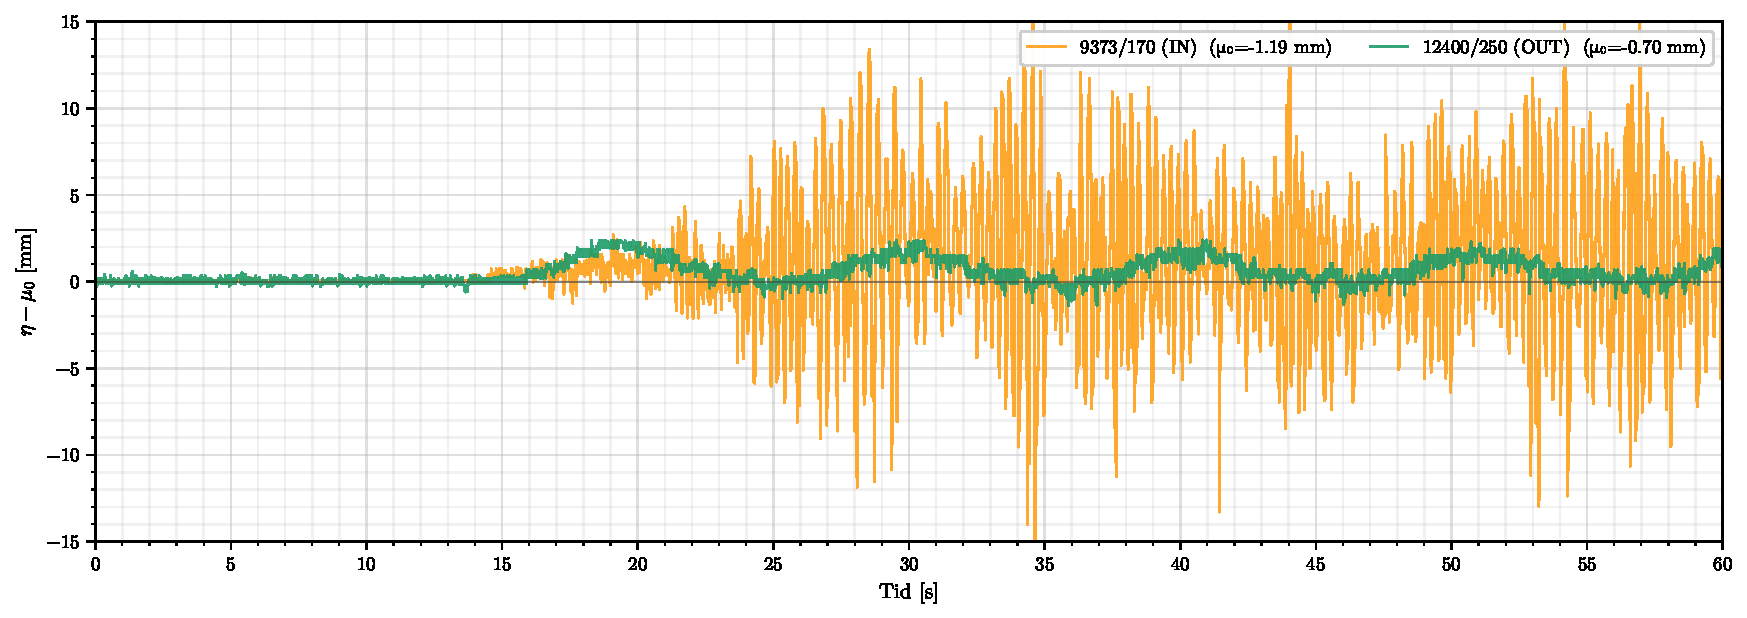
\includegraphics[width=\linewidth]{FIGURES/ch04_wind_rampup_zoom60.pdf}
    \caption{TODO}
    \label{fig:ch04_wind_rampup_zoom60}
  \end{subfigure}
  \\[1ex]
  \begin{subfigure}[b]{1.0\linewidth}
    \centering
    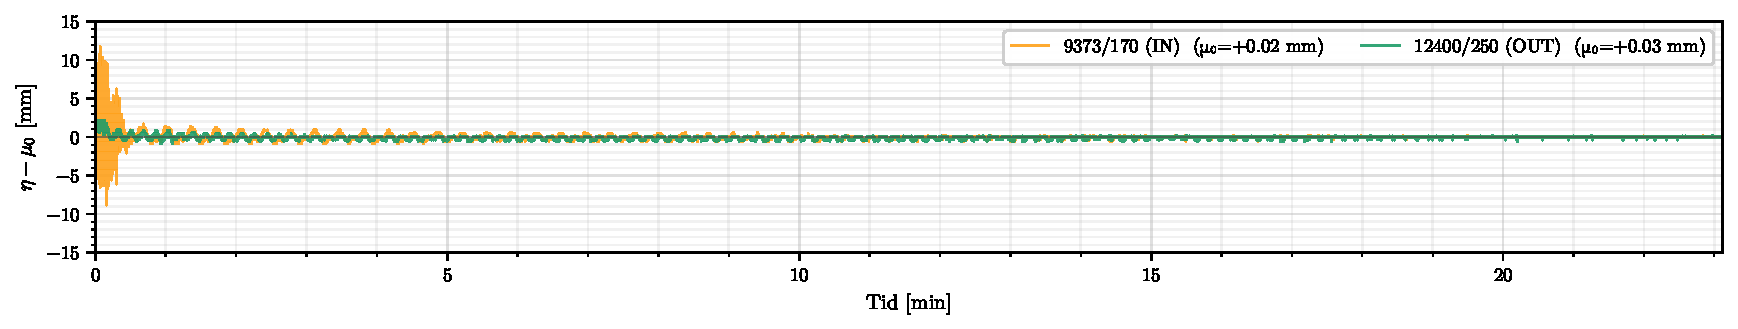
\includegraphics[width=\linewidth]{FIGURES/ch04_wind_decay_full.pdf}
    \caption{TODO}
    \label{fig:ch04_wind_decay_full}
  \end{subfigure}
  \\[1ex]
  \begin{subfigure}[b]{1.0\linewidth}
    \centering
    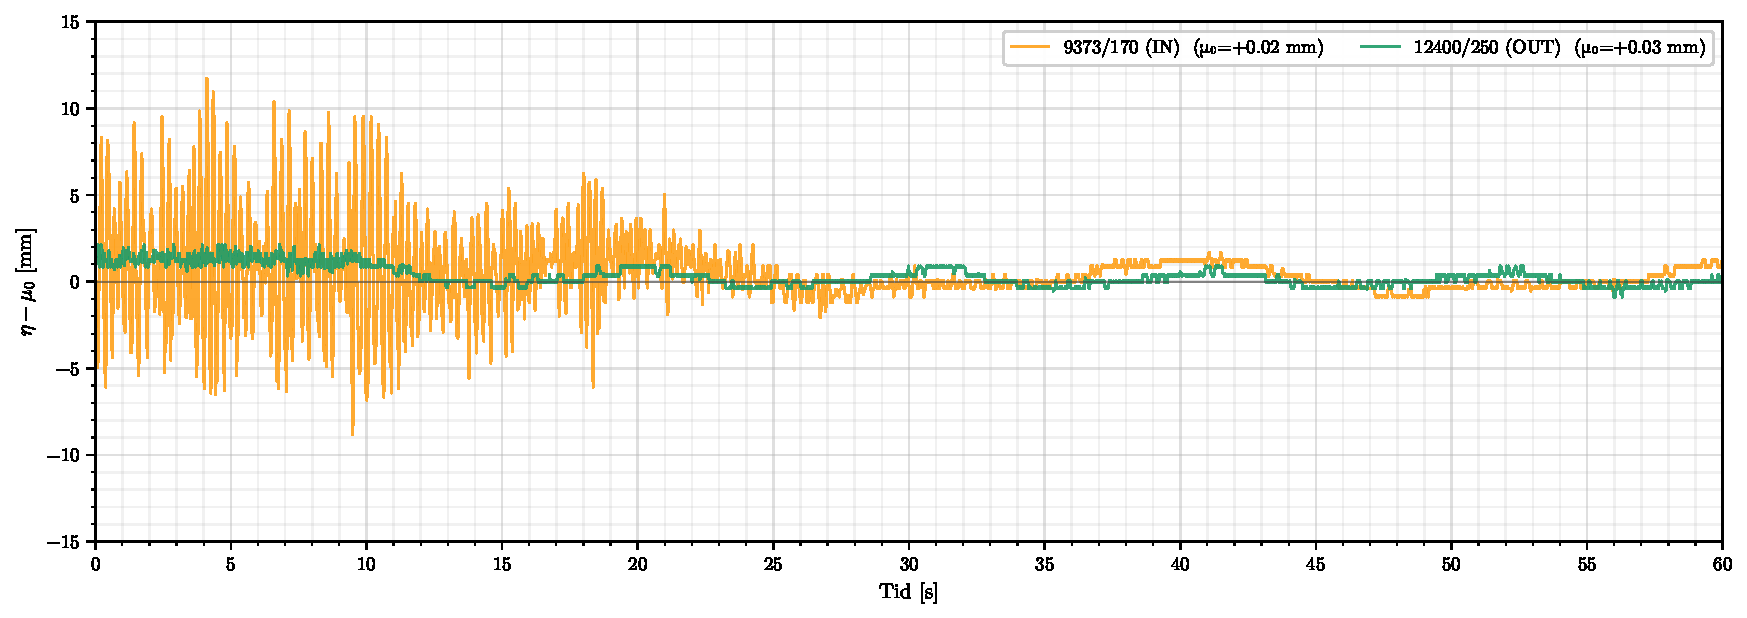
\includegraphics[width=\linewidth]{FIGURES/ch04_wind_decay_zoom60.pdf}
    \caption{TODO}
    \label{fig:ch04_wind_decay_zoom60}
  \end{subfigure}
  \caption{
    % TODO: write caption
  }
  \label{fig:ch04_wind_transition_overview}
\end{figure}
